\documentclass[tikz]{standalone}
\usepackage{pgfplots}
\pgfplotsset{compat = newest}

\begin{document}
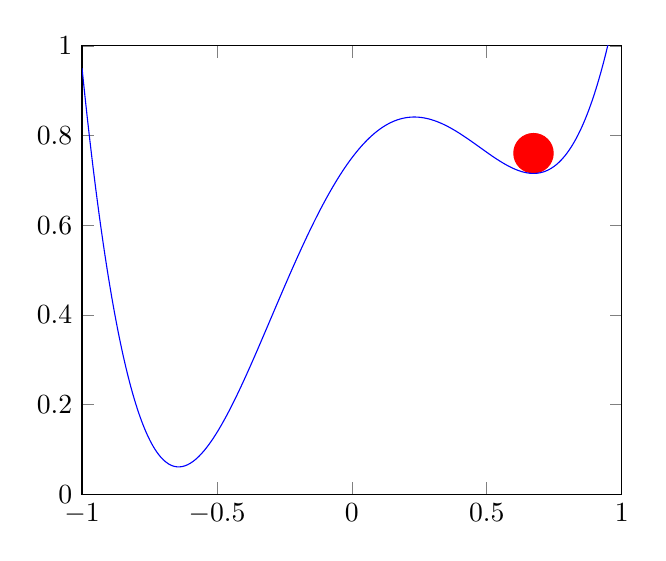
\begin{tikzpicture}
  \begin{axis}[xmin=-1,xmax=1,ymin=0,ymax=1]
    \node[circle,draw=red,fill=red,minimum size = 0.5cm,anchor=south] at (0.67317,0.71533){}; %minimum size = diameter of the circle.
    \addplot [thin,samples=200,smooth,blue,domain=-1:1] {2*x^4-0.7*x^3-1.7*x^2+0.8*x+0.75};
  \end{axis}
\end{tikzpicture}
\end{document}